\chapter{Historical Social Network Analysis Process, Pitfalls, and Network Modeling}\label{ch:hsna-process-and-network-modeling}
\minitoc

I describe in this chapter a formalization of the \hsna workflow followed by social historians, to shed light on their process and summarize recurring pitfalls to identify how \va could support them in this workflow.
Most \hsna practitioners report on their findings concerning the network they constructed from their sources, but few highlight the process which led to these conclusions from the raw historical documents, even though they have to make several encoding, modification, and modeling decisions that deeply influence the final analysis\cite{alkadi2022}.
Specifically, social historians can model documents and their content through various network models which have been proposed in the literature.
I discuss this step in depth as it impacts the annotation and analysis possibilities, and I give an answer to our first research question \qone by proposing to model this type of data with \modelplural.
This model satisfies \simplicity, \reality, and \traceability properties, which we define as critical for social history work from our joint collaborations with social historians and current critics of \hsna \cite{lemercier12FormalNetwork2015, lemercierBackSourcesPracticing2021, edelsteinHistoricalResearchDigital2017}.

\paperbox{This chapter is an updated version of an article presented at the VIS4DH workshop of the IEEE VIS: Visualization \& Visual Analytics Conference 2022 which is currently being published in IEEE Explore\cite{pisterHistoricalDocumentsSocial2022}. It was a collaboration with Nicole Dufournaud, Pascal Cristofoli, and my supervisors Christophe Prieur and Jean-Daniel Fekete. I have been leading the discussions, elaboration of concepts, and writing of the paper.}

\section{Context}

Tools for social network visualization tend to ignore the context in which the networks are produced, where they come from, and the workflow that led from their origin (e.g., documents, polls, interviews, web scraping) to their network form.
Yet, practitioners of social history need to inspect and encode their sources in depth using ad hoc methods to generate a network, and sometimes end with errors or simple networks which do not fit their analysis goals\cite{lemercierQuantitativeMethodsHumanities2019}.
%Yet, practitioners of social history need to generate many networks from the same documents/sources to visualize and analyze them
% and need to maintain the provenance from documents to analyzes and back.
% In this article, we explain why and how effective tools for supporting Historical Social Network Analysis~\cite{wetherell_historical_1998} (HSNA) should model social networks in multiple steps to support three essential principles: \traceability, connection to \emph{reality}, and \simplicity.
In this chapter, after describing and characterizing the workflow of \hsna~\cite{wetherellHistoricalSocialNetwork1998} from our collaborations with social historians, I explain why and how effective tools for supporting this process should model social networks in multiple steps to support three essential principles: \traceability, \reality, and \simplicity.
These principles emerged from joint experiences as historians and computer scientists were collaborating on multiple projects, and aim at simplifying the \hsna process while enhancing exploration and analysis options and replicability.
%These principles emerged from joint experiences as historians and computer scientists while collaborating on multiple projects, and aim at simplifying the \hsna process while enhancing exploration and analysis options and replicability.

Social historians' goal is to characterize socio-economic phenomena and their dynamics in a restricted period and place of interest and to see how individual people of that time lived through those changes\cite{tilly1984retrieving}.
For this, they rely on historical documents that they inspect in depth to next extract qualitative and quantitative information allowing them to answer their research questions.

%They typically extract qualitative and quantitative information from an identified corpus of documents, to then make conclusions on socio-economic topics such as migrations, business dynamics, education, and kinship.
%For doing this, historians can apply Social Network Analysis (SNA), a method---sometimes referred to as a paradigm---which consists in modeling the social relationships between a set of entities---usually individuals---into a network.
%Much work has been done to adapt SNA to the context of historical document exploitation, and although several approaches coexist they can be brought together under the banner of Historical Social Network Analysis~\cite{wetherellHistoricalSocialNetwork1998} (HSNA) or Historical Network Research~\cite{kerschbaumerPowerNetworksProspects2015} (HNR).
To study relational social structures where individuals influence each other such as families, companies, and institutions, historians rely on \hsna by modeling the social relationships between a set of entities---usually individuals---into a network.
%Historians therefore collect documents, annotate them, construct a network from the annotations that they finally analyze and visualize to understand the structural aspect of their object of study by validating and/or generating new hypotheses.
However, the process leading to the final network from the raw documents is often linear, and it is common that, when visualizing their network, historians spot errors and inconsistencies in the network structure that they could have fixed if the process was more iterative\cite{alkadi2022}.
Moreover, historical documents are often complex, meaning that the annotation and modeling process can be done in many different ways, concerning what to annotate from the documents\cite{lemercierBackSourcesPracticing2021} and how to model the annotation in a network\cite{cristofoliAuxSourcesGrands2008}.
Several network models have been proposed ranging from simple and specific ones like co-occurrence networks to more general and complex ones such as multilayer networks and knowledge graphs.
Simple models allow answering specific questions and are easy to manipulate but are often too simplistic and may distort the information contained in the documents.
Moreover, they often break the traceability from the analysis to the original documents, making the communication of findings less reproducible and the process of modifying/correcting annotations complicated.
Indeed, errors and mismatches often occur in the annotation process, for example, due to entity disambiguation problems\cite{diesnerImpactEntityDisambiguation2015}.
On the contrary, too complex models are complicated to visualize and analyze, and historians do not always have the tools to create them properly.
In this chapter, I answer \qone (how to model historical documents into analyzable networks with the right balance between expressivity and simplicity) by proposing to model historical documents as \modelplural, where both persons and documents are modeled as nodes with attributes and the links represent both individuals' mentions in the documents and their social roles in the event witnessed by the documents (such as witness in a marriage act).
While this model is simple enough for creation and inspection, it allows tracing back the entities of the network to the original sources for a continuous annotation process and still accurately models the social relationships mentioned in the documents.
Historians can therefore use this model to simultaneously find errors and inconsistencies in their annotation process---allowing them easier back and forth between the annotation and analysis steps---while starting a first analysis and exploration of the data to answer their sociological questions.
The traceability to the original sources also makes the communication of findings more replicable and transparent.

% Very often, historians model the persons mentioned in the text as the nodes of the network, who are connected two by two by links modeling social relationships, such as friendships and family ties.
% However, historical documents are often rich in information and can refer to complex relationships involving more than two persons at the same time. Persons can also have different implications or roles in the documents, and relationships are often non symmetrical~\cite{lemercier_analyse_2005}.
% For example, there have been several studies on business documents concerning financial transactions~\cite{rossi_exploration_2014, crailsheimSpanishConnectionFrench2016}. These documents often involve more than two persons, who can have  different roles; this type of documents refer to sellers and buyers, but can also indicate other roles such as a guarantor, witness, or notary. These complex relationships are hard to model into simple person-to-person networks.
% Furthermore, textual sources almost always contain extra information in regard of the event they refer to like the date and time, location, and other such as the type and amount of the transactions. It can also contain extra information about the persons such as their job, family, and gender.
% It is clear that such information-rich data is difficultly modeled as a simple person-to-person network. Yet, even if more complex models have been proposed in the literature such as dynamic and bipartite networks, simple networks are still the most widespread model supported by popular tools.
% Moreover, a large number of HSNA studies focus on reporting network analysis results, but rarely give details on the encoding, annotation, and network modeling process even though these are primordial steps which influence greatly the final results. Therefore, it can be difficult for readers to trace back the analysis to the original documents, and can pose replicability problems~\cite{baker_1500_2016}. For these reasons, network models that can more faithfully represent the complex reality of the documents while allowing traceability to the sources and are easy enough to manipulate are needed.
% In this paper, we first describe the HSNA work process that we have observed from the literature and collaborations, starting from the textual sources acquisition to the analysis and visualization of the network, and we identify potential issues related to analysis for each step.
% Then, after describing the most used network models in HSNA, we formalize a network model which satisfies \textit{reality} and \traceability properties, and
% which models well the majority of historical sources we encountered with their complexity: the \model. We give real world examples on how this model has been used to follow HSNA pipelines, from data preparation to visual analysis using a visual query system. From these examples, we identify three problems which arise when doing a network projection but not when using \modelplural: no loss of information, no duplication, and no distortion.

%
%\section{Related Work}
%
%Since we already elaborated on the related work of SNA, HNR, network modeling, and social network visualization in \autoref{ch:related-work}, we only discuss in this section the related work concerning historians' workflow and methodology descriptions.
%
%The essence of the historical discipline is based on a critical approach of sources and involves considering peers' work.
%Traditional approaches to history often focus on the construction of a narrative, without necessarily adopting a systematic and problematized approach to the exploitation of original sources.
%Social history and the ``Annales School'' proposed a new approach to history, by trying to describe and characterize socio-economic phenomena of the past by rigorously extracting information from historical documents and making conclusions from them.
%
%
%
%With similar aims, Glaser and Strauss developed the ``Grounded Theory''~\cite{glaserDiscoveryGroundedTheory2010} as a methodology for the humanities to build hypotheses and theories by solely studying and categorizing real-world observations, without starting from prior knowledge and predefined categories.
%Later on in the 1960s, quantitative methods started to be used in history, providing statistical and later computer-supported tools to aid historians in grounding their analysis in mathematical models and results.
%Unfortunately, the lack of methodology and understanding between the two worlds led to many criticisms by historians pointing to using wrong metrics, simplifying categories, and disconnections between the original documents and analysis~\cite{karila-cohenNouvellesCuisinesHistoire2018, lemercierBackSourcesPracticing2021}.
%Quantitative history has been showed to be useful when used properly and when not focusing only on numbers, and several books have been published on how to efficiently use statistical methods such as summarizations, correlations, statistical distributions, statistical testing, time series etc.~\cite{hudsonHistoryNumbersIntroduction2016, lemercierQuantitativeMethodsHumanities2019}.
%Similarly, the use of network science for historical aims increased in recent years, and a lot or resources exist on how to use network methods and measures for historical research~\cite{lemercier12FormalNetwork2015, kerschbaumerPowerNetworksProspects2015}.
%
%However, little work has been done on describing and formalizing the process before the analysis part for a quantitative and network research workflow.
%Indeed, if it is central to know how to manipulate statistical and network concepts and methods when following this kind of methodology, it is as important if not even more to follow a correct and rigorous workflow to generate the data we plan to analyze beforehand.
%The process to generate a clean quantitative or network dataset from historical sources is difficult and requires several data acquisition, annotation, and cleaning steps.
%Social analysts are not always trained on how to do these steps effectivity, which can lead to errors, inconsistencies, and mismatches between the chosen data models and the historical questions~\cite{alkadi2022}.
%Karila-Cohen and al.\ provide some advice on how to annotate historical documents with the aim of using quantitative methods~\cite{karila-cohenNouvellesCuisinesHistoire2018} and prone that the annotation and analytical processes should not be dispatched between several persons, as both usually influence each other.
%Dufournaud describes her workflow in depth when studying the socio-economic status of women in France in the 16th and 17th centuries, which she splits into three steps: \textit{data collection}, \textit{data processing}, and \textit{data analysis}~\cite{dufournaudCommentRendreVisible2018}.
%She provides the tools and methodology she used to annotate her data, providing transparency on her historical analysis and methodological resources.
%Cristofoli discusses the network modeling problem when following an HSNA and highlights the fact that the same historical documents can be modeled in different ways~\cite{cristofoliAuxSourcesGrands2008}.
%Historians should be aware of this and choose a network model which fits their analytical goals.



\section{Related Work}

Since I already elaborated on the related work of SNA, network modeling, and social network visualization in \autoref{ch:related-work}, I only discuss in this section the related work concerning historians' methodology and workflows.

%\subsection{Methodologies and formalisms}

\subsection{History Methodology}

%The essence of the historical discipline is based on a critical approach of sources and involves considering peers' work.
%Traditional approaches to history often focus on the construction of a narrative, without necessarily adopting a systematic and problematized approach to the exploitation of an exhaustive set of historical documents.
%Social history and the ``Annales School'' shifted the focus from a narrative approach of History focused on individuals, towards exhaustive inspection of documents to make sociological conclusions on groups and organizations.
%Historians therefore started to extract numbers and categories from their sources to point to social and economical aspects of societies. \todo{example}
%This type of practice logically led historians to use quantitative methods with the rise of computer science in the 1960s.


The essence of the historical discipline is based on a critical approach to sources and involves considering peers' work.
Traditional approaches to history often focus on the construction of a narrative, without necessarily adopting a systematic and problematized approach to the exploitation of an exhaustive set of historical documents\cite{tillyObservationsSocialProcesses2004}.
With the development of social and quantitative history, historians now have a panoply of methods to exhaustively extract quantitative data from their sources and analyze it to ground their results in verifiable claims.
Many historians criticized this computational aspect of history\cite{lepetitHistoireQuantitativeDeux1989, fogelLimitsQuantitativeMethods1975, barnesBigDataLittle2013}, pointing out that it would lead to errors and missing the core content of historical sources.
However, using quantitative approaches and formalisms is not exclusive to having a deep understanding of the documents and their context, nor building a narrative on top of their quantitative analysis.
Good historical work can in fact be described as a combination of the two \cite{karila-cohenNouvellesCuisinesHistoire2018}, as Tilly says ``Formalisms play their parts in the space between the initial collection of archival material and the final production of narratives. In my own historical research, formalisms figure prominently from early in the ordering of evidence to late in its analysis; \textup{[\,\dots]} As it happens, many other historians rush from sources to reasoned narratives without pausing to employ formalisms, or even to reflect very self-consciously on the logical structure of their arguments, hence on what the evidence should show if their arguments are correct'' \cite{tillyObservationsSocialProcesses2004}.
Historians have a panoply of methods and formalisms they can leverage to ground their narratives in concrete comparable results, such as serial analysis, tabular analysis, classical statistical treatments, and network analysis.

However, formalisms have to be used wisely and with a critical vision of the documents and their context, so as to not fall into simplifications, anachronisms, and errors which are pertinent critics of quantitative history\cite{lemercierQuantitativeMethodsHumanities2019, lemercierBackSourcesPracticing2021}.
%Such formalisms often demand categorization and aggregation of the original documents, which can result in distortion and simplification of the original documents content \cite{lemercierQuantitativeMethodsHumanities2019}.
Most historical work leverage several methods in the same study to support their claims through different qualitative and quantitative results \cite{petzCombiningNetworkResearch2022}.
The level of the plausibility of a claim increase or decrease depending on if the different evidence point to similar results or not.
%If several different evidence point to the same fact, the level of plausibility of the claim increase, even without uing formal statistical testing.
Similarly, historians often work on small populations or specific individuals---as it is the case with microhistory studies\cite{ginzburgMicrohistoire1981}---which can result in complications for generalization.
Only after studying several similar individuals or groups, historians are able to generalize and point to exceptions.
For example, by comparing several Jewish commercial communities in Europe during the first half of the 18th century, Trivellato has been able to generalize what is common to those groups (they have been trading between them and with outer ethnic groups) and what is specific to each (such as their business strategies) \cite{trivellatoThereFutureItalian2011}.
%Most historical work do not go to the level of statistical testing to verify their claims, but often combine several formalisms with a narrative to refute or support a hypothesis.
%As the objects of study are often on small to medium groups, the combination of several studies lead to the increase or decrease of level of plausibility of different claims.


%\todo{Grounded Theory}



\subsection{Historian Workflows}

%Many approaches have been introduced to analyze historical documents through various formalisms to analyze their content through quantification.
Many quantitative methods and formalisms are available for historians to inspect their sources with the aim of making historical claims.
Several textbooks describe and explain to social scientists and students who do not have formal computer science training in what consist these methods (statistical regression, Chi-squared test, network analysis, etc.) and how to practically use those with software and programming language \cite{archdeaconCorrelationRegressionAnalysis1994, floudIntroductionQuantitativeMethods2013}.
However, the process leading from the sources to the numeric artifacts (a table, a network, a timeline) has not been described thoroughly in the literature, especially with concrete examples, and is often not presented in scientific publications of concrete use cases.
Yet, the process leading from the documents to analyzable data requires social historians to make several annotations, encoding, and modeling decisions, concerning \emph{what} to extract from the source and \emph{how} to encode it.
This process is tedious and requires data acquisition, annotation, encoding, and modification with continuous back and forth between the different steps \cite{alkadi2022}.
%The process to generate a clean quantitative or network dataset from historical sources is difficult and requires several data acquisition, annotation, and cleaning steps.
%Social analysts are not always trained on how to do these steps effectivity, which can lead to errors, inconsistencies, and mismatches between the chosen data models and the historical questions~\cite{alkadi2022}.
This is a critical process as it can lead to simplifications, anachronism, distortion, or data that do not allow to answer original or new hypotheses \cite{karila-cohenNouvellesCuisinesHistoire2018, lemercierQuantitativeMethodsHumanities2019}.
Lemercier et al. give guidelines on how to encode information from historical documents to prevent introducing bias, by having a critical view of the documents \cite{lemercierBackSourcesPracticing2021}.
They emphasize the importance of the input phase of research and advise copying the first documents by hand while characterizing them in the most exhaustive and factual way, without imposing categorization.
This explorative step lets historians familiarize themselves with the content of the document, leading to a better view of what to encode to answer their research questions and sometimes to the formulation of new hypotheses.
For example, in their project on the social and geographical trajectories of Jews in Lubartów\cite{zakrzewski1932PopulationRegister2020}, a village in Poland, the team encoded the mean of writing inside the register documents (pen, pencil, ink, etc.) they were inspecting.
This information  allowed them to conclude that the inscription ``expelled'' written in pencil was probably added during World War II by Germans to denote exported Jews in the extermination camps.
When applying network analysis, historians often create specific person-to-person networks which allow them to answer precise research questions, but often lose this type of document-related information.
% If historians decide to apply network analysis, they also have to decide how to model their network, based on the entities they can extract from their documents and their research questions.
Cristofoli discusses the network modeling problem when following a network analysis and highlights the fact that the same historical documents can be modeled in different ways~\cite{cristofoliAuxSourcesGrands2008}, which can result in mismatches between the network shape and the research questions.
Dufournaud presents her quantitative and network workflow when studying the economic role of women during the 16\ts{th} and 17\ts{th} centuries in the city of Nantes, which she splits into three steps: data collection, data processing, and data analysis \cite{dufournaudCommentRendreVisible2018}.







%With similar aims, Glaser and Strauss developed the ``Grounded Theory''~\cite{glaserDiscoveryGroundedTheory2010} as a methodology for the humanities to build hypotheses and theories by solely studying and categorizing real-world observations, without starting from prior knowledge and predefined categories.
%Later on in the 1960s, quantitative methods started to be used in history, providing statistical and later computer-supported tools to aid historians in grounding their analysis in mathematical models and results.
%Unfortunately, the lack of methodology and understanding between the two worlds led to many criticisms by historians pointing to using wrong metrics, simplifying categories, and disconnections between the original documents and analysis~\cite{karila-cohenNouvellesCuisinesHistoire2018, lemercierBackSourcesPracticing2021}.
%Quantitative history has been showed to be useful when used properly and when not focusing only on numbers, and several books have been published on how to efficiently use statistical methods such as summarizations, correlations, statistical distributions, statistical testing, time series etc.~\cite{hudsonHistoryNumbersIntroduction2016, lemercierQuantitativeMethodsHumanities2019}.
%Similarly, the use of network science for historical aims increased in recent years, and a lot or resources exist on how to use network methods and measures for historical research~\cite{lemercier12FormalNetwork2015, kerschbaumerPowerNetworksProspects2015}.
%
%However, little work has been done on describing and formalizing the process before the analysis part for a quantitative and network research workflow.
%Indeed, if it is central to know how to manipulate statistical and network concepts and methods when following this kind of methodology, it is as important if not even more to follow a correct and rigorous workflow to generate the data we plan to analyze beforehand.
%The process to generate a clean quantitative or network dataset from historical sources is difficult and requires several data acquisition, annotation, and cleaning steps.
%Social analysts are not always trained on how to do these steps effectivity, which can lead to errors, inconsistencies, and mismatches between the chosen data models and the historical questions~\cite{alkadi2022}.
%Karila-Cohen and al.\ provide some advice on how to annotate historical documents with the aim of using quantitative methods~\cite{karila-cohenNouvellesCuisinesHistoire2018} and prone that the annotation and analytical processes should not be dispatched between several persons, as both usually influence each other.
%Dufournaud describes her workflow in depth when studying the socio-economic status of women in France in the 16th and 17th centuries, which she splits into three steps: \textit{data collection}, \textit{data processing}, and \textit{data analysis}~\cite{dufournaudCommentRendreVisible2018}.
%She provides the tools and methodology she used to annotate her data, providing transparency on her historical analysis and methodological resources.
%Cristofoli discusses the network modeling problem when following an HSNA and highlights the fact that the same historical documents can be modeled in different ways~\cite{cristofoliAuxSourcesGrands2008}.
%Historians should be aware of this and choose a network model which fits their analytical goals.


\section{Historical Social Network Analysis Workflow}\label{sec:hsna-workflow}


From the literature and our own projects of \hsna we conducted during the last three years in collaborations with social historians, I propose a formalization of the \hsna workflow divided into 5 steps: \textit{textual sources acquisition}, \textit{digitization}, \textit{annotation}, \textit{network creation}, and finally, \textit{visualization and analysis}.
I start by describing the sources and research questions of the different collaborations in \autoref{subsec:hsna-examples}, then explain each step of the workflow in \autoref{subsec:hsna-workflow}, and characterize three properties \va systems supporting this workflow should satisfy in \autoref{subsec:hsna-properties}.
%The workflow is presented in \autoref{fig:HSNA-process} along with potential and recurrent pitfalls.


\subsection{Examples}\label{subsec:hsna-examples}

We discussed with four experienced social historians collaborators at different steps of their \hsna workflow about their process: how they inspect and annotate their sources, what network representation they plan to use, and what are their research questions.
%annotation process and how they wanted to model their data into a network.
They all work on semi-structured historical documents, mentioning complex relationships.
I provide more details in the following:

\begin{enumerate}[nosep,leftmargin=*]
    \item Analysis of the social dynamics from \textbf{construction contracts in Italy in the 18\ts{th} century\cite{Cristofoli2018, Rolla2018}.}
    %\textcolor{red}{PC: The corpus was created by N. Rolla through the exploitation of the manuscript registers of the \textit{Azienda generale fabbriche e fortificazioni} (State Archives of Turin)[REF : Rolla Nicoletta, 2018, "Mobilité et conflits. Travailler sur les chantiers de construction piémontais dans la première moitié du XVIIIe siècle" dans Andrea Caracausi et Marco Schnyder (eds.), Travail et mobilité en Europe (XVIe-XIXe siècles), Villeneuve d’Ascq, Presses universitaires du Septentrion (coll. Histoire et civilisations), p. 49‑72]. }
    The corpus is made of contracts for different types of constructions in the Piedmont area in Italy. People are typically mentioned under three different construction roles: \textit{Associates} who are in charge of the construction, \textit{Guarantors} who bring financial guarantees, and \textit{Approvers}, who vouch for the guarantors. Documents contain information about the building sites, the types and materials of constructions, and the origins of people. Historians working on this project were interested in characterizing the social structure underlying those contracts, if there were specializations in types of construction, and describing the life trajectory of certain people.
    \item Analysis of migrations from the \textbf{genealogy of a French family between the 17\ts{th}--20\ts{th} centuries} [unpublished work].
    The corpus is made of family trees referring to several document/event types: birth and death certificates, marriage acts, military records, and census reports.
    The social historian wants to characterize the main migrations of individuals and families in France, according to time and place.
    She is also interested in studying specific families, with theories that, in some areas, people were moving places in a circular fashion over the years.
    Finally, she is interested in the average social mobility of individuals across the years.
%    The roles are different for each event type and consist of \textit{children, father, mother} for the birth events, \textit{deceased} for the death event, \textit{spouse} and \textit{witnesses} for the marriages, and \textit{family member}s for the census events.
    \item Analysis of \textbf{marriage acts in Buenos Aires in the 17--19\ts{th} centuries ~\cite{moutoukiasBuenosAiresPort2016, rueda1989matrimonios}.}
% \textcolor{red}{PC: The corpus was created by Z. Moutoukias \& C. Prieur through the digitization and annotation of a publication of the Buenos Aires Archives [REF: Jauregui Rueda, Carlos, Matrimonios de la catedral de Buenos Aires, 1747 – 1823, Buenos Aires, Fuentes Genealógicas e Históricas Argentinas, 1989]. }
    The corpus is made of summaries of marriage records that mention the spouses and the witnesses of the wedding.
    The origin, date of birth, and parents' names are specified for both spouses.
    The historian is mainly interested in characterizing the relationships between witnesses and spouses---if they are typically from the same family, and if being a witness is sometimes used to ask favors in exchange.
    % These parenting relationships are important for our collaborator, but do not refer to the same event as the marriage. Thus, we create another event node referencing the birth event, with \textit{father, mother}, \textit{child} as roles and the associated birth year and location as node attributes.
    \item Socio-political analysis of \textbf{Germans ethnic migration from communist Romania to West Germany in the 20th century (ongoing work)~\cite{diminescuMigrationEthnicGermans2020}.}
    The corpus is made of administrative forms that mention persons requesting to migrate, along with the persons they want to join, and the administrative persons of the ministry in charge of the forms.
    The family members of the aspiring migrants are also mentioned in the forms, with their respective dates of birth.
    Our historian collaborator is interested in characterizing the socio-economical profile of migrants and the types of family members they are typically joining in Germany.
\end{enumerate}

Each historian planned to follow a network analysis.
They typically first read and inspect their sources in depth, before encoding their content with the aim of constructing a network.
They plan to use analytical and visualization tools to then explore the structure of the relationships, and answer their questions.

\subsection{Workflow}\label{subsec:hsna-workflow}

\begin{figure}
%    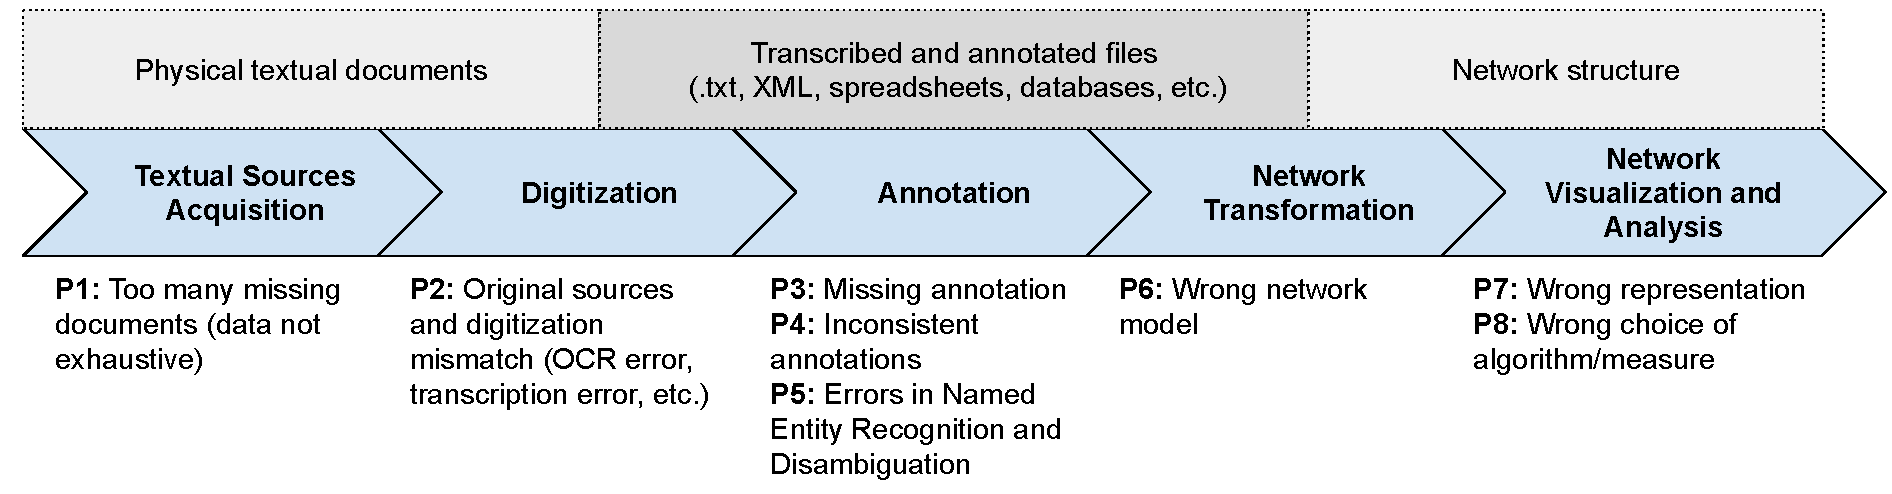
\includegraphics[origin=c, width=\textwidth]{static/figures/HSNAProcess/OriginalPaperFigures/Process5.pdf}
    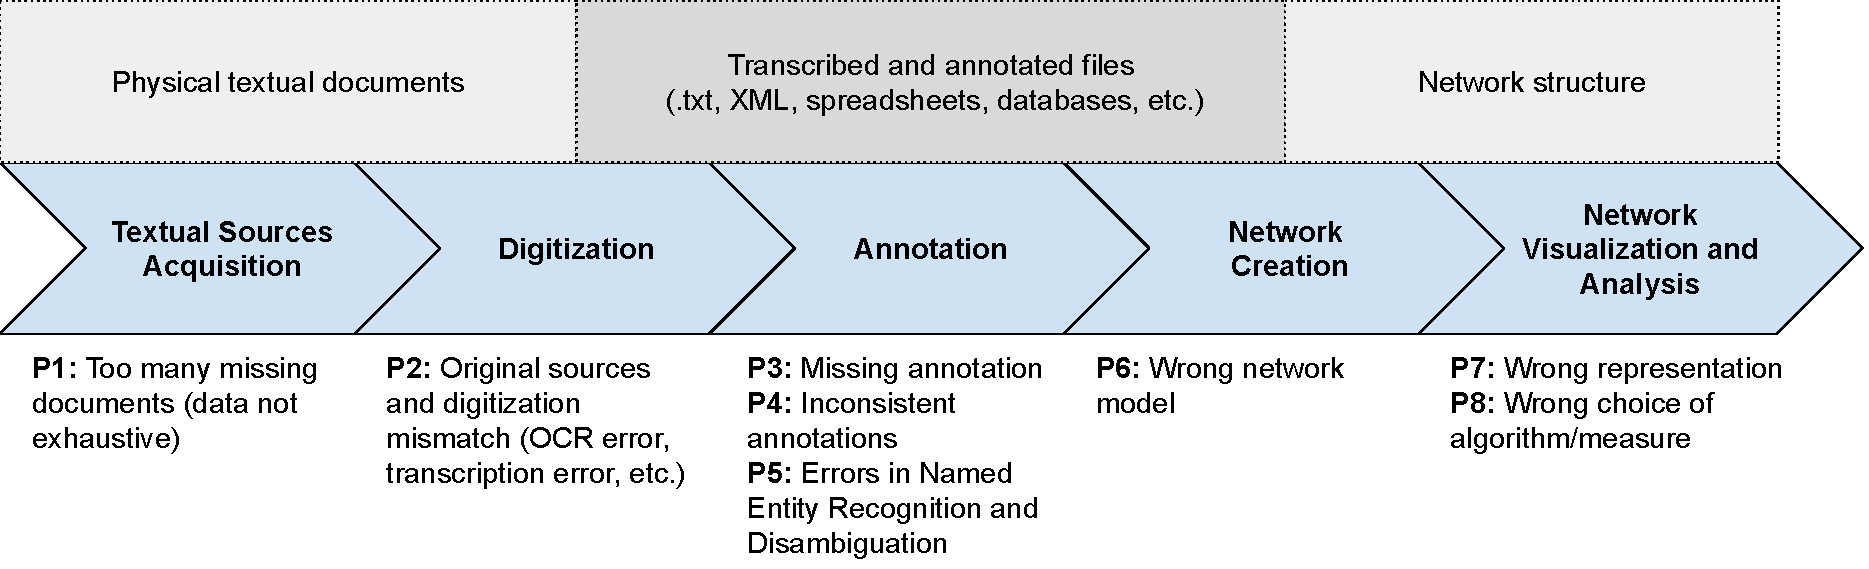
\includegraphics[origin=c, width=\textwidth]{static/figures/HSNAProcess/process.pdf}
    \caption{HSNA workflow is split into five steps: textual sources acquisition, digitization, annotation, network creation, and network visualization/analysis. Practitioners typically have to do back and forth during the process. I list potential pitfalls for each step.}
    \label{fig:HSNA-process}
\end{figure}

% This process is not straightforward, and has not been discussed a lot in the HSNA community. Dufournaud describes her workflow when studying socio-economic status of women in France in the 16th and 17th centuries, that she split in three steps: \textit{data collection}, \textit{data processing}, and \textit{data analysis}~\cite{dufournaud2018comment}. From the literature and discussions with historians collaborators we propose an HSNA workflow description split in 5 steps: \textit{textual sources acquisition}, \textit{digitization}, \textit{annotation}, \textit{network creation} and finally \textit{visualization and analysis}. The workflow is presented in \autoref{fig:HSNA-process} along recurrent potential issues which can arise.
%\noindent\textbf{Textual Sources Acquisition}

I formalize the \hsna workflow of social historians from our collaborations (\autoref{subsec:hsna-examples}) but also the literature, and informal discussions with other social historians.
We can divide it into 5 steps: \textit{textual sources acquisition}, \textit{digitization}, \textit{annotation}, \textit{network creation}, and finally, \textit{visualization and analysis}.
For each step, I present recurring pitfalls which occurred during our collaborations, or that are discussed in the literature\cite{diesnerImpactEntityDisambiguation2015, cristofoliAuxSourcesGrands2008, lemercierAnalyseReseauxHistoire2005}.
A diagram of the workflow is presented in \autoref{fig:HSNA-process}.

%\subsubsection{Textual Sources Acquisition}
\noindent\textbf{Textual Sources Acquisition}
Historians' first step is gathering a set of textual historical documents mentioning people with whom they will have social ties.
For this, they usually take documents from a specific source---such as a folder from a national or local archive---and restrict them to a period and place that they want to study.
They also often restrict themselves to one document type---such as marriage or notary acts---to focus the analysis on one or a few types of social relationships that they want to understand in depth.
However, one rule of the historian's method is to crosscheck from multiple sources, so an initial corpus is often extended with another set of related sources.
Once they restricted their search to a set of documents, a time, and a geographic area, they try to exhaustively find all the documents matching the desired properties, as \textbf{missing documents can result in uncertainty in the network structure and, therefore, the sociological conclusions (P1)}.

%\subsubsection{Digitization}
\noindent\textbf{Digitization}
Digitization consists in converting the sources into a digital format.
% \textcolor{green}{For modern history where the documents have been produced digitally or scanned and digitized through optical character recognition (OCR), this step can be skipped. For modern documents, digitization is now almost always done as it allows to tremendously ease the storage, indexation, and annotations of the documents} \textcolor{red}{
This step can be skipped for the most recent periods where many documents have been produced digitally or can be scanned and well digitized through optical character recognition (OCR), allowing tremendous ease in the storage, indexation, and annotation of the documents.
%, and facilitates the creation of a network object afterwards.
% is the only accessory step of the process, as everything can in theory be done without a computer,
However, before mid 20\ts{th} century, most historical primary sources are stored in archives in paper format and need human work to be digitized.
However, most historical primary sources originated before mid 20\ts{th} century are stored in archives in paper format and need human work to be digitized.
% Digitization can be done by hand or with the help of Optical Character Recognition (OCR) tools.
\textbf{Mismatches between the original documents and the transcription can occur for old and recent documents (P2)}.
However, if OCR tools are more and more efficient in English and highly used languages, historians can work with old documents written in old or extinguished languages and with atypical writings (e.g., Fraktur handwriting and typefaces for German in the early 20\ts{th} century).
Therefore, OCR tools are often unusable in social history, and digitization remains an expensive and sometimes highly skilled process.

%\subsection{Annotation}
\noindent\textbf{Annotation}
Annotation (often called \emph{encoding}) is the process of finding and extracting useful information from the documents concerning the persons, their social ties, and any useful information for the historian.
This extra information can concern the persons (their age, profession, sex, ethnicity, etc.) and their social relationships (type, date, place).
It encompasses \emph{named-entity recognition} as well as their resolution.
Historians also sometimes annotate information on other entities mentioned in the documents, such as art objects or administrative entities.
Usually, historians have a first idea of what they want to annotate in the data as they already explored the documents beforehand and have knowledge of their subject of study, with hypotheses they want to explore.
It is, however, common they change their mind through the annotation process, by reflecting on what they found in the documents.
Unfortunately, this can produce \textbf{missing annotations (P3)} and \textbf{inconsistent annotations (P4)} at the end of the process if annotators are not careful.
This task can also be challenging, and the choice of annotations has an impact on the final network.
Historians also face ambiguity in the process, as several persons and entities (like cities) can have the same name (homonyms), refer to a place name that has disappeared (street name or city), or to an ambiguous person (e.g., John Doe).
They, therefore, have to follow a NER and resolution/disambiguation process to identify entities in the sources and disambiguate them across several documents.
Entity resolution has always been a problem in social history---as it is more generally in text analysis, where typical groundwork consists in crossing information about the same entities from different heterogeneous sources.
However, errors in the disambiguation process can lead to important distortions in the final network structure and properties~\cite{diesnerImpactEntityDisambiguation2015}, e.g, people connected to the wrong ``John Doe''.
Historians usually carry out this process manually but can also use automated methods and refine the results themselves later.
Unfortunately, \textbf{errors are common in this step as automated methods do not provide perfect accuracy, nor do doing it manually given the lack of global information (P5)}.\\
The Text Encoding Initiative (TEI)~\cite{TEI} is an XML vocabulary and a set of guidelines typically used to encode and annotate documents, and the events happening in these documents (unclear parts, gaps, mistakes, etc.).
It is also used for historical texts and to generate social networks~\cite{dufournaudComparaisonOutilsPour2006, serranomolineroUnderstandingUseVistorian2017}.
Unfortunately, the guidelines are not meant to define a canonical annotation, and different persons can interpret the guidelines in different ways, leading again to inconsistent annotations of corpora (P4) and to errors or distortions in social networks derived from these annotations.
% Several softwares can be used for annotation and are usually stored in markups formats such as XML .

%\subsection{Network Creation}
\noindent\textbf{Network Creation}
Historians construct one or multiple networks from the annotations of the documents.
Typically, all persons mentioned are annotated and are transformed into network nodes (vertices).
Additional information, such as their age, profession, and gender, can be stored as node attributes.
How the network's links are created is not as trivial and can vary from project to project~\cite{alkadi2022}.
The most straightforward approach is to create a link between every pair of persons mentioned in one document, thus forming a clique motif.
This is a simplistic heuristic as social relationships can be quite complex, involving more than two persons who can have different roles in the relationship.
The choice of the network model has a major impact on the future analysis and \textbf{may add bias if chosen loosely (P6)}, such as the creation of network structural artifacts when using network projections\cite{cristofoliAuxSourcesGrands2008}.
More complex models have been proposed in the literature, such as weighted, dynamic, bipartite, and layered networks, but can be hard to manipulate and visualize. I discuss them more in detail in \autoref{sec:modeling}.

%\subsection{Network Analysis and Visualization}
\noindent\textbf{Network Analysis and Visualization}
Once historians have constructed a satisfactory network, they start exploring and analyzing it with visualization and quantitative methods.
The final goal of HSNA is to find interesting patterns and link them to social concepts to gain high-level socio-historical insights~\cite{freemanDevelopmentSocialNetwork2004, wetherellHistoricalSocialNetwork1998}.
Usually, historians start to visualize their network to visually confirm information they know and to potentially gain new insight with exploration.
Representations need to be chosen wisely given the network as lots of techniques and tools exist for social network visualization. \textbf{Some insight may be seen only with some specific visualization technique (P7)}.
To test or create a new hypothesis, historians typically rely on algorithms and network measures.
Lots of network measures have been developed, like modularity, centrality, and clustering coefficient, that social scientists can leverage to make conclusions~\cite{scottSocialNetworkAnalysis1988}.
Similarly, social scientists can use data mining algorithms to highlight interesting and potentially hidden structures in the network, \eg by using clustering algorithms revealing group structures~\cite{brandesModularityClustering2008}.
\textbf{However, they have to interpret the results carefully (P8)} as some algorithms act as black boxes and some measures are hard to interpret, with unclear sociological meaning (e.g., centrality).
Typically, particular patterns and measure values in the network could have different potential sociological meanings.
If we take as an example betweenness centrality which measures the number of times a node appears in the shortest path of every pair of existing nodes, individuals with high values usually highlight positions of power as they communicate with different groups.
However, it can also be interpreted as a position of vulnerability in other contexts, such as during periods of wars and repressions, as in the study of Polish social movements in the 20th century by Osa~\cite{osaSolidarityContentionNetworks2003}, where she shows persons with high betweenness centrality values are more targeted for repression in certain periods.
Social scientists, therefore, have to be careful when interpreting network measures and take into account the globality of their sources when interpreting the network they constructed.


\subsection{Visual Analytics Supported Historical Social Network Analysis}\label{subsec:hsna-properties}

Social historians typically follow the workflow described in \autoref{subsec:hsna-workflow} linearly, meaning that at the end of the process, they can realize that the analysis and visualization of the network do not allow them to answer their research questions\cite{lemercier12FormalNetwork2015}.
This can, in part, be explained by the fact that visualization and analytical \sna tools are only focused on the last part of the process.
To fully support social historians, \va interfaces should therefore provide assistance and guidance on the whole process, from the acquisition of the documents (since archives now provide digital collections that can be explored through visualization\cite{forliniMiningMaterialArchive2018, thudtBohemianBookshelfSupporting2012}) to the final analysis.
Specifically, from discussions with our collaborators, we identify three properties that \va interfaces should satisfy for good integration into the historians' workflow and to limit the recurring pitfalls we identified in \autoref{subsec:hsna-workflow}: \traceability, \reality, and \simplicity.
\begin{figure}[!ht]
    \centering
    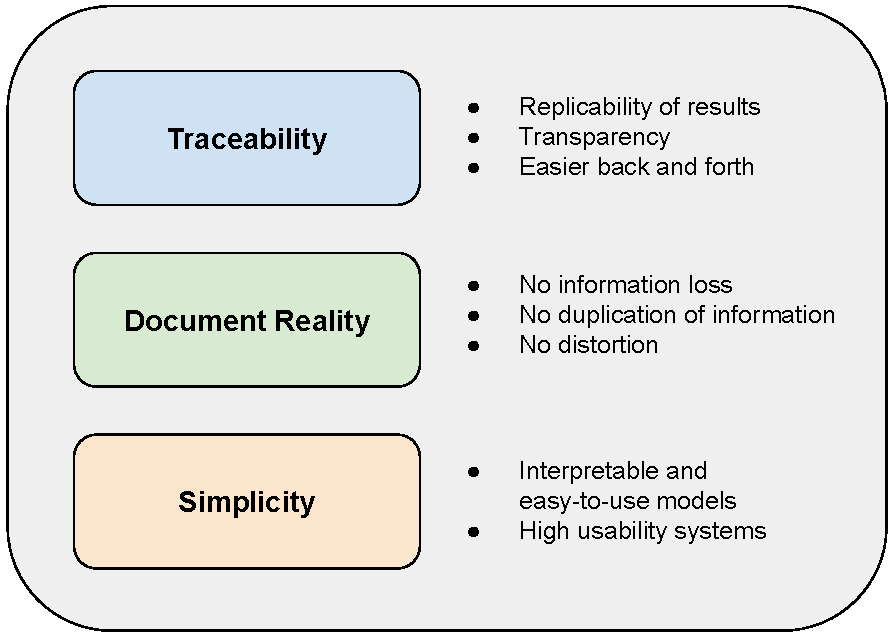
\includegraphics[width=0.70\linewidth]{static/figures/HSNAProcess/properties}
    \caption{Three properties essential to \va systems supporting the social historians workflow: \traceability, \reality, and \simplicity.}\label{fig:HSNA-properties}
\end{figure}
First, Traceable systems enable to do easier back and forth between the different annotation, modification, modeling, and analysis steps and provide a transparent chain of operations leading from the acquisition of the sources to the high-level socio-historical conclusions.
Traceability should be operated during the annotation and modeling process (for example to see why two mentions of persons have been given the same identifier, and to trace back network entities to the documents' annotations) but also during exploration.
Seeing every low-level operation (filter, selection, group-by, etc.) leading to the generation of insight leads to better transparency and replication\cite{callahanVisTrailsVisualizationMeets2006, xuSurveyAnalysisUser2020}.
Second, the digitization, encoding, modeling, and analysis/visualization steps should always reflect the textual reality of the documents \ie the \reality\footnote{We chose the term ``document reality'' over simply ``reality'' after a conversation with a historian to highlight the fact the historical documents do not describe factually the reality and reflect the subjective bias of the context in which the person wrote them\cite{karila-cohenNouvellesCuisinesHistoire2018}. The content of the documents, therefore, has to be modeled by taking into account this context, which can reveal interesting behaviors and structural patterns. See \cite{lemercierBackSourcesPracticing2021} for specific examples.}, in order to reduce the introduction of bias, simplification, and anachronisms in the analysis\cite{karila-cohenNouvellesCuisinesHistoire2018, lemercierQuantitativeMethodsHumanities2019}.
Indeed, encoding and modeling the data with abstraction and constructed concepts\footnote{In anthropology, the terms \emph{emics} and \emph{etics} refer respectively to intrinsic phenomena related to observation and constructed categories and abstractions\cite{headlandEmicsEticsInsider1990}.} such as the concept of families or ``social proximity'', often result in distortions (simplification or modifications), duplication, and loss of information contained in the documents.
Specifically, the choice of the network model embodies how the content of the sources is manipulated and abstracted with the goal of making historical conclusions, and deeply influences the annotation/encoding and analysis/visualization steps.
I discuss network models more in depth in the next \autoref{sec:modeling}.
Finally, as discussed in \autoref{sec:intro-HSNV}, social scientists often have trouble importing their data in \sna tools\cite{alkadi2022} and often perform ``soft SNA''\cite{rollingerProlegomenaProblemsPerspectives2020} only due to usability problems and ``Math anxiety''\cite{paxtonDollarsSenseConvincing2006}.
\va tools should therefore focus on \simplicity through the use of simple and comprehensible models and high usability systems.
The three properties and their effects on the workflow are summarized in \autoref{fig:HSNA-properties}.





\section{Network Modeling and Analysis}\label{sec:modeling}

% \subsection{Quantitative History}

% Traditionally, historians try to tell a story about protagonists and socio-economic facts in a given society. This narrative approach of history have been criticized for its lack of traceability and the open interpretation of historical documents, which can introduce bias from the author.
% Social history and HSNA brought answers to this problem by bringing quantitative methods to enforce a narrative supported by data and statistical results. However, traditional HSNA studies describe globally their sources without precising the annotation and transformation process they followed. They don't mention how the network they study has been obtained from the sources. Yet, these steps are critical as they can deeply influence the results of the analysis~\cite{lemercier_analyse_2005}~\cite{cristofoli_aux_2008}. Indeed, historians have to make choices on what to annotate and what to model into the network. This often depends on what they want to demonstrate at the end.
% As these steps of the workflow are often not transparent, it can be difficult for the reader of an HSNA study to understand how does the network has been constructed, what it represents, and to trace back the network entities from the original sources~\cite{dufournaud2018comment}~\cite{dufournaud_recherche_2015}.

% Recently, Experimental Computer Science went through a replicability crisis, pointing out that a lot of results were not reproducible, since authors were not giving enough data or information for people to redo the same analysis. Reproducibility is though considered a condition for building scientific knowledge, and this discussion highlighted the fragility of a lot of experimental studies. Data shows that the natural and social sciences are also affected~\cite{baker_1500_2016}.

% Usage of computer science in history can mitigate this problem, by providing methods and tools for historians to follow their analysis and providing traceability from their high level conclusions to the original documents.

% We argue one way of doing that is to use a network model which reflects well the \textbf{reality} of the social relationships mentioned in the documents, and are \textbf{traceable} to the original sources. We think network models which satisfy these two properties---\textbf{reality} and \textbf{traceability}---should always be constructed from the original sources as a basis for the analysis. Other network transformations can be applied afterwards to reveal specific patterns, but having a network which reflects well the reality of the documents is primordial for representing the sources as they are, and allowing to easily go back to them at any point in the analysis. Indeed, any transformation can be applied from a network representing well the sources. But applying modifications and transformations directly in the annotation process can bias the analysis and remove the possibility to follow other explorations and hypothesis in the future.

% Indeed, historians have to make choices on what to annotate and what to model into the network. This often depends on what they want to demonstrate at the end.
% As these steps of the workflow are often not transparent, it can be difficult for the reader of an HSNA study to understand how does the network has been constructed, what it represents, and to trace back the network entities from the original sources~\cite{dufournaud2018comment}~\cite{dufournaud_recherche_2015}.

% When transforming the information of the documents into a network, historians have to make choices on what to annotate and what to model into the network. As these steps of the workflow are often not transparent, it can be difficult for the reader of an HSNA study to understand how does the network has been constructed, what it represents, and to trace back the network entities from the original sources~\cite{dufournaudCommentRendreVisible2018}. Also, too complicated models are harder to visualize and analyze. For these reasons, we argue that a good network model should reflects well the reality of the social relationships mentioned in the documents, is traceable to the original sources, and is simple enough to visualize and understand.
% We think network models which satisfy these three properties---\textbf{reality},  \textbf{traceability} and \textbf{simplicity}---should always be constructed from the original sources as a basis for the analysis.

Historians typically construct one or several networks from their annotated documents that they visualize and analyze to validate or find new hypotheses.
As the processing steps of the workflow are often not transparent (digitization, annotation, network modeling), it can be difficult for the reader of an \hsna study to understand how the network has been constructed, what it represents, and to trace back the network entities to the original sources~\cite{dufournaudCommentRendreVisible2018}.
Moreover, visualizing the network very often highlights errors and artifacts of the annotations, along with potential mismatches between the network model and the analysis goals.
Historians then have to correct or change their annotations, even though it is a very tedious and demanding process to repeatedly switch back and forth between the network and the annotated documents.
Several network models make the task harder as they do not directly represent the documents, and it is thus difficult to relate a network entity to a specific document and annotation.
Therefore, I believe that more \va tools should support social scientists in annotating and modeling their documents to make the HSNA process less linear by allowing easier back and forth between the annotation, modeling, and visualization steps.
Network models satisfying  \traceability, \reality, and \simplicity properties would mitigate those problems by allowing to navigate more easily between the network and the documents while still modeling well the social relationships mentioned in the sources and being easy enough to visualize and manipulate for analytical and data modification goals.
%the data and detect potential errors and inconsistencies.

The choice of the network model to represent the social relationships mentioned in historical documents deeply influence the annotation and visualization/analysis processes.
Many network types have been proposed in the literature.
While simple ones---which are widely used---are easy to manipulate, they very often break \traceability---the network entities are not traceable to direct annotations, and sometimes correspond to constructed concepts---and the \emph{reality} of the documents.
On the contrary, complex models are often hard to manipulate and visualize.
I present the most widely used network models in the \hsna literature in \autoref{subsec:hsna-network-models} and present \modelplural as a model satisfying those three properties in \autoref{subsec:hsna-bipartite-model}.

\subsection{Network Models}\label{subsec:hsna-network-models}

Currently, historians use various network models depending on their knowledge of network science, the content of their documents, the schema of their annotations, and the analysis they plan to make. By ``model'' I refer to a mapping from the historical documents to a graph mathematical model and its semantic, \ie what the network entities represent in terms of sociological concepts (for example simple networks and co-occurrence networks have the same simple graph model $G = (V, E)$ but with different semantics).
I describe here the most used network models in \hsna along with more recent ones:

\begin{itemize}[nosep,leftmargin=*]
    \item \textbf{Simple networks~\cite{wetherellHistoricalSocialNetwork1998}:} According to their research hypotheses, historians select and merge document information to build a specific relationship between individuals. They analyze this simple network structure with \sna tools and produce network indicators and node-link visualizations. It is often difficult to connect the results to the original sources. Moreover, it does not take into account the diversity of social relationships, as every link is identical.
    \item \textbf{Co-occurrence networks~\cite{sairioMethodologicalPracticalAspects2009}:}
    % rubio-mondejarWomenEntrepreneursFamily2022}: % , keekMovementPerspectivesCollective, bouletBatchKernelSOM2008
    Only the persons are represented as nodes, and two persons are connected with a link when they are mentioned in the same document (or section). This can be a useful model to detect community-related patterns, but the constructed notion of ``proximity'' represented by the links simplifies and hide the diversity of social relationships.
    \item \textbf{Multiplex Unipartite Networks~\cite{eriksonMalfeasanceFoundationsGlobal2006}:} Only the persons are represented as nodes, and links model social ties between two persons. Links can have different types representing different types of social relationships. It allows the modeling of more complex social relations where people can have various social ties e.g. as parents, friends, and business relationships. However very often several possible representations for the same data exist as projections are often applied to the original documents to get this type of model.
    %, and very often several possible representations for the same data exist, especially for complex relationships. [jdf] true for the other network types
    \item \textbf{Bipartite/two-mode networks\footnote{Bipartite refers to the mathematical property that nodes of the network are split between two sets without any links between two nodes of the same sets, while the term two-mode refers to networks modeling two types of entities.}~\cite{hambergerScanningPatternsRelationship2014}
    %~\cite{hamberger_scanning_2014, lippPetitionsSocialContext2001a, shafie_hypergraph_2017}
    :} Nodes can have two types: persons and documents in this network model. A link refers to a mention of a person in a document and can thus only occur between a person and document nodes. Usually, links are not typed and only encode mentions.
    More recent analyses in \hsna encode the \emph{roles} of the persons in the documents as link types~\cite{Cristofoli2018}. This network model is more aligned with the original sources and allows following an analysis through the original documents themselves and not through concepts. It can also be used to represent constructed concepts, like the GEDCOM format which introduces the concept of ``family'' that ties together a husband, spouse, and children with different link types.
    The concept of family can have different meanings across time and cultures, meaning that GEDCOM adds a conceptual layer instead of grounding the network to concrete traceable documents and events (e.g., no marriage but birth certificates).
    % In our model, a family tie would be replaced by different documents: the marriage certificate and  birth certificates, to ground the network to concrete traceable documents and events.
    \item \textbf{Multilayer networks~\cite{multilayer}: } In these networks, each node (vertex) is associated with a \emph{layer} $l$ and becomes a pair $(v, l)$, allowing to connect vertices inside a layer or between layers. These advanced networks have received attention from sociologists~\cite{CRNOVRSANIN201456} and historians~\cite{vanVugt_2017}, but they are complex. The meaning of a layer varies from one application to another; it can be time (years), type of documents, the origin of sources, etc. They, therefore, offer many (too many) options for modeling a corpus, and visualizing it, with no generic system to support historians for taming their high complexity.
    \item \textbf{Knowledge graphs~\cite{hoganKnowledgeGraphs2021}: } they represent knowledge as triples $(S, P, O)$ where $S$ is a \emph{subject}, $P$ is a \emph{predicate}, and $O$ is an \emph{object}. Everything is encoded with these triples using controlled vocabularies of predicates and rules known as \emph{ontologies}. Knowledge Graphs are popular for encoding knowledge on the web, including historical knowledge. However, it is notoriously complex to encode documents using knowledge graphs due to the complexity of the format and the wide choice of possible ontologies. Most historians are unable to understand knowledge graphs and even less to use them for annotating a corpus. Since knowledge graphs are generic, they need complex transformations to be visualized, with no generic system to support historians in taming their high complexity.
\end{itemize}


%\autoref{fig:HSNA-network-models} shows a schematic representation of the different network models.
%We can rank the models given two axes: simplicity/complexity and specificity/expressiveness.
%Currently, historians mostly construct unipartite networks (simple, co-occurrence, and weighted) which are simple and allow them to answer specific questions.
%However, those models do not capture all the complexity of the documents and social scientists may miss important patterns.
%For example, modeling only co-occurrences of persons in documents remove the variety of social relationships these mentions can refer to~\cite{lemercier12FormalNetwork2015}.
%Several interpretations may coexist to explain why someone is central in the resulting network, which may be impossible to validate without encoding more information---such as the types of relationships---in the model.
%Depending on the schema of the annotations, it may be impossible to create more complicated networks at this step without redoing the annotation process which is costly in time and resources.
%On the contrary, too complicated models such as KG are difficult to create from the sources and are hard to visualize and analyze, especially for social scientists who are not trained in those kinds of formalisms.
%Using this kind of model usually requires learning complex query language to manipulate the data, such as the SPARQL language for KG\@.
%Therefore, we argue that historians should aim to model a network that is simple enough to manipulate, can be traced back to the original sources, and model well the social reality of the documents---i.e. having those three properties: \simplicity, \traceability, and \textit{reality}.

%We argue that historians should aim to model their networks simply enough to be manipulated by them, in a way that entities can be traced back to the sources, and expressive enough to model accurately the social reality of the documents---i.e., having those three properties:  \simplicity, \traceability, and \reality.

Currently, most digital history projects use one-mode networks (simple, co-occurrence, and multiplex) that are simple and allow answering specific questions, but they do not capture all the complexity of the documents, resulting in simplifications and distortions of the structural patterns.
I compare what would be the resulting networks for these models and the bipartite model of our three collaboration use cases (the example \dana is still in the phase of data acquisition), with additional information from the documents encoded as node and link attributes.
I do this for one given document for each dataset.
The results are shown in \autoref{tab:models}.

\begin{table}[!ht]
    \begin{tabular}{|m{4.5cm}|m{2.7cm}|m{2.7cm}|m{2.7cm}|}
        \hline Original Document & Co-occurrence            & Unipartite Multiplex    & Bipartite           \\
        \hline \tiny \underline{1712}: Construction of a church in \underline{Torino}.
        Associates: \colorbox{associate}{Bellotto G, Bello P.M, Bello G.}
        Guarantor: \colorbox{guarantor}{ Astrano G.A.}
        Approbator: \colorbox{approbator}{Corte A.} \linebreak
        \colorbox{associate}{Associate} \colorbox{guarantor}{Guarantor} \colorbox{approbator}{Approbator}
        & \centering\simplePiemont & \centering\unipartitePiemont & \bipartitePiemont   \\
        % \hline Le 7 octobre 1901, \colorbox{father}{François Marie Esnault} et \colorbox{mother}{Marie Julie Léopoldine Colson} ont déclaré la naissance de leur fille, nommée \colorbox{child}{Blanche Esnault} dans la commune de Saint-Maur-des-Fossés.uuu
        \hline \tiny Du \underline{dix-neuf fevrier mil huit cent quatre-vingt quatre}, à six heures du soir.
        Acte de naissance de \colorbox{child}{Dufournaud Alexis, enfant de sexe masculin} né le \underline{dix-neuf février}, à deux heures du soir au \underline{village de Grudet, commune de Saint} \underline{Symphorien}, des mariés \colorbox{father}{Dufournaud Alexis}, \colorbox{father}{cultivateur colon, âgé de trente ans}, et \colorbox{mother}{Marie Pardonnaud,} \colorbox{mother}{sans profession, agée de vingt-six ans}, demeurant au village de Grudet, dite commune de Saint-Symphorien. [...]
        \linebreak
        \colorbox{father}{Father} \colorbox{mother}{Mother} \colorbox{child}{Child}
        & \centering\birthSimple   & \centering\birthUnipartite   & \birthBipartite     \\
        \hline % \centering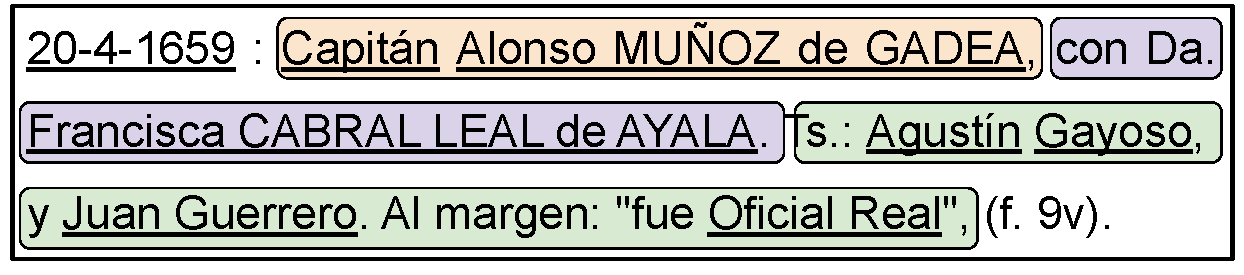
\includegraphics[scale=0.3]{OriginalPaperstatic/figures/HSNAProcess/OriginalPaperFigures/marriageDocumentnoParents}
        \tiny \underline{20-4-1659} : \colorbox{epoux}{\underline{Capitán} Alonso MUÑOZ de GADEA}, con Da. \colorbox{epouse}{Francisca CABRAL LEAL de AYALA}. Ts.: \colorbox{temoin}{Agustín Gayoso}, y \colorbox{temoin}{Juan Guerrero. Al margen: "\underline{fue Oficial Real}"}, (f. 9v). \linebreak
        \colorbox{epoux}{Husband} \colorbox{epouse}{Wife} \colorbox{temoin}{Witness}
        & \centering\simple        & \centering\noParents         & \bipartiteNoParents \\
        \hline
    \end{tabular}
    \caption{Resulting networks using different models produced by one document of the examples detailed in \autoref{subsec:hsna-examples}: co-occurrence, unipartite and bipartite models. The first column shows the partial transcription of real documents (simplification for collaboration \pascal). Colors represent annotations concerning the persons mentioned, their roles, and their attributes. Underlines refer to information related to the events and which can be encoded as document/event attributes.
    Only time is represented for simplification, but other attributes would follow the same schema.
    H: Husband, W: wife, T: Witness, M: Marriage, $A_N$: Associate, G: Guarantor, Ap: Approbator, C: Construction, F: Father, M: Mother, C: Child.
    }\label{tab:models}
\end{table}

As shown by Cristofoli~\cite{cristofoliAuxSourcesGrands2008}, we can clearly see the co-occurrence model removes the complexity of the social relationships and only show an abstract ``proximity'' between individuals.
Unipartite multiplex networks allow producing meaningful networks which model well the diversity of relations that can link several people.
It especially models simple relationships well, such as parenting ones as in example \nicole.
However, it produces distortions for more complex relationships involving more than two persons, as in example \pascal where people can either be mentioned as associates, guarantors, and approbators in the documents.
Associates should probably be linked together with \textit{associate} links, but the \textit{guarantors} and \textit{approbators} relationships are more complex to model.
Approbators could be linked to the associates, the guarantors, or both.
The three ways of modeling this type of relationship make sense but can lead to very different network shapes and analysis results.
Historians thus have to decide on a transformation among several possibilities, which will probably distort the social reality of the relationships.

These examples also show that when working with multivariate networks, using projections to create unipartite networks brings a duplication of information.
Indeed, if a document mentions information like a date that we model as an attribute, we can store it as a document node attribute using a bipartite model.
However, when projecting the network, this information appears in the links as many times as there are persons mentioned in the document minus one and often more.
For example, in the example \pascal in \autoref{tab:models}, the time of the construction is stored in $\sum_{i=1} ^{4} i = 10$ links in the co-occurrence model and in 9 links in the multiplex unipartite model, while it is only stored once as a document node attribute in the bipartite model.

Both co-occurrence and unipartite multiplex models thus do not satisfy the \reality property by introducing constructed concepts---such as abstract notions of ``proximity''---or inferring one-to-one social relationships from mentions in a document mentioning more than two actors.
Moreover, projections add ambiguity in retrospect of the original documents, as it becomes impossible to trace back one link to one specific document, as the same link could potentially refer to several ones~\cite{cristofoliAuxSourcesGrands2008}, \ie they do not satisfy the \traceability principle.

More complex models, such as multilayer networks and knowledge graphs, could satisfy \reality and \traceability principles (depending on the modeling choices, as these models are very expressive and do not enforce specific data schemas) but are complex to manipulate and visualize, especially for social scientists.
In contrast, the bipartite model satisfies the \reality and \traceability properties through the representation of documents as nodes, and individuals' mentions as links encoding their roles.
This model is simple enough to manipulate according to the number of \sna studies leveraging it \cite{lippPetitionsSocialContext2001, shafieHypergraphRepresentationsStudy2017, davisDeepSouthSocial2009, ochabDetectingOttokarII2022} and the development of \sna bipartite measures and algorithms\cite{borgattiSocialNetworkAnalysis2009, latapyBasicNotionsAnalysis2008, hambergerScanningPatternsRelationship2014}.
Yet, most \hsna studies are based on the network topology and often do not leverage attributes, including time and location.
We, therefore, claim that \modelplural allow to model historical documents with \traceability, \reality, and \simplicity properties.
I formalize and describe this model in the next \autoref{subsec:hsna-bipartite-model}.

%For example, modeling only co-occurrences of persons in documents remove the variety of social relationships these mentions can refer to\cite{lemercier12FormalNetwork2015}.
%Moreover, since documents are not explicit in the unipartite model, it is hard to trace the network entities back to the sources: the traceability property is not satisfied, meaning that the data is harder to correct and that analyses are less replicable.
%On the other side, multilayer networks and knowledge graphs allow to model documents as entities and express complex relationships between various other entities they mention.
%These models can be very expressive but are challenging to use for historians, especially without guidelines; without \simplicity, the \traceability and \reality properties can be hard to achieve.
%The lack of simplicity, therefore, results in difficulties for visualization and analysis, especially for social scientists.


% TODO: maybe to a better figure
%\begin{figure}
%    \centering
%    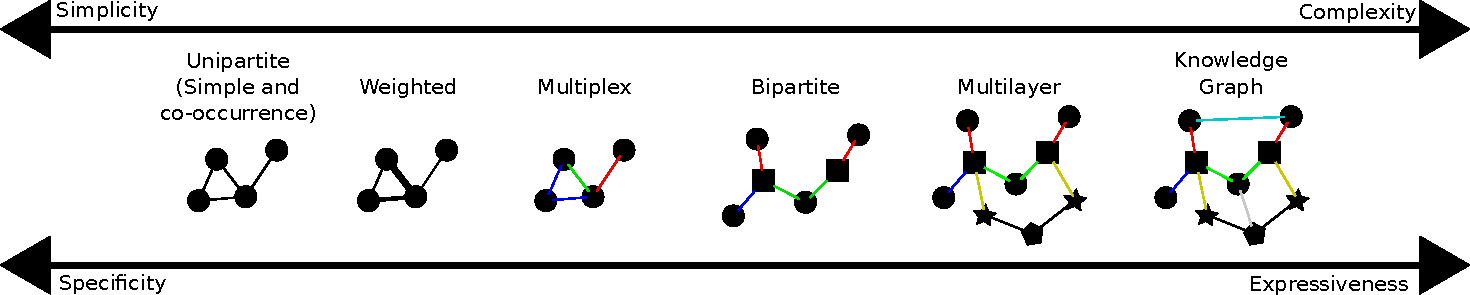
\includegraphics[width=\columnwidth]{static/figures/HSNAProcess/OriginalPaperFigures/models.pdf}
%    \caption{Schematic representations of Different network models used for analyzing historical documents, ordered by complexity and expressiveness}
%    \label{fig:HSNA-network-models}
%\end{figure}

%\autoref{fig:HSNA-network-models} shows a schematic representation of the different network models, ranked on simplicity/complexity and specificity/expressiveness axis.


% \begin{table}
% \centering
% \resizebox{\columnwidth}{!}{%
% \tiny
% \begin{tabular}{|l|l|l|l|}
% \hline
%                               & Traceability & Reality & Simplicity \\ \hline
% Simple Networks               & \xmark       & \xmark  & high       \\ \hline
% Co-occurrence Networks        & \xmark       & \xmark  & high       \\ \hline
% Multiplex Unipartite Networks & \xmark       & \xmark  & high       \\ \hline
% Bipartite Networks            & \cmark       & \cmark  & medium     \\ \hline
% Multilayer Networks           & \cmark       & \cmark  & low       \\ \hline
% Knowledge Graphs              & \cmark       & \cmark  & low  \\ \hline
% \end{tabular}%
% } \caption{Network models table.}
%  \label{tab:HSNA-modelsAndProps}
% \end{table}

\subsection{Bipartite Multivariate Dynamic Social Network}\label{subsec:hsna-bipartite-model}

Historical documents are well modeled by bipartite multivariate dynamic networks with roles, that can be formalized as

\begin{equation}
    G = (V, E, B, R, T, L)
\end{equation}

where $V$ is the set of vertices, $E$ the set of edges, and $B = {person, document}$ the set of node types.
Each node $u \in V$ is defined as

\begin{equation}
    u = (u_{id}, b_u, a_u)
\end{equation}

where $u_{id}$ corresponds to the unique identifier of $u$, $b_u \in B$ is the type of the node and $a_u$ is a tuple of the attributes (or properties) values of $u$. If $b_u = person$, then

\begin{equation}
    a_u = (a_i, \dotsc, a_N)
\end{equation}

with $a_i, \dotsc, a_N$ the attributes values of the node $u$ of the $N$ attributes defined on person nodes, defined on their domains $A_i, \dotsc, A_n$.
Document nodes always have a time and location such that for a document node $v \in V$  with $b_v = document$ then

\begin{equation}
    a_v = (t, l, a_i, \dotsc, a_M)
\end{equation}

with $t \in T$ is the time of the event witnessed by the document, $l \in L$ its location, and $a_i, \dotsc, a_M$ the attributes values of the node $v$ of the $M$ attributes defined on document nodes (other than time and location), defined on their domains $A_i, \dotsc, A_M$.
Similarly, each edge $e \in E$ is defined as

\begin{equation}
    e = (u, v, r, a_e)
\end{equation}

with $u, v$ the vertices connected by $e$ such that $b_u \neq b_v$, $r \in R$ the role of the person mentioned in the document and $a_e$ the attributes tuple of $e$ such that

\begin{equation}
    a_e = (a_i, \dotsc, a_O)
\end{equation}

with $a_i, \dotsc, a_O$ the attributes values of the edge $e$ of the $O$ edge attributes defined on their domains $A_i, \dotsc, A_O$.

The model has, therefore, the following properties:
\begin{description}[nosep,leftmargin=2mm]
    \item[{Bipartite:}] There are \textbf{two types of nodes}, persons and documents (or events). An event, such as a marriage, is most of the time witnessed by a document, and we refer to them interchangeably as events and documents. Events considered in the network can be of the same sub-type, such as contracts, or of multiple subtypes, \eg for genealogy: \emph{birth certificates}, \emph{death certificates}.
    \item[Links and Roles:] A link models the mention of a person in a document. \textbf{Each link has a type corresponding to the role of the person in the document}. For a marriage act, the roles include \emph{wife}, \emph{husband}, and \emph{witness}. This is a key aspect of our model since it clarifies the relationship between the persons within an event. In contrast, Jigsaw~\cite{staskoJigsawSupportingInvestigative2008} does not consider the roles.
    \item[{Multivariate:}] Each entity of the model can have attributes, that give additional information. Person nodes are referenced by a key that reflects the disambiguation process. They can have general information (standardized name, gender, birth date). Documents are also identified by a key, \eg an archive reference. The associated event can have a date, a location, and potentially other information. Links can also carry information to describe contextual properties (activity, residence, etc.).
    \item[{Geolocated:}] Events should have a location when it makes sense, ideally with the longitude and latitude.
    \item[{Dynamic:}] Events are always dated. We rely on this date since it encodes the social dynamics of the network.
\end{description}

One of the main benefits of this model is that the document nodes represent both the physical documents and the events the documents refer to.
For example, concerning marriage acts, the document nodes represent both the physical documents with their texts but also the marriage events with their characteristics modeled as attributes (time, location, etc.).
Therefore, social historians can use this model to store, process, and annotate their original documents and follow an analytical workflow with the same representation.
This model is \textit{simple} enough to manipulate and visualize for historians and allows tracing back every entity of the network to the documents according to the \traceability principle.
Still, the network preserves the \reality of the social relationships mentioned in the sources as no projection or transformation is applied.

Visualization tools using this model can focus on the topology of the network, and/or the attributes which I express here in the format of tuples, commonly used by databases and visualization systems\cite{stoltePolarisSystemQuery2002}.
However, it has to be taken into account that if the attributes extracted from the historical documents are related to vertices and edges independently to the topology of the network, it can be appropriate to compute vertices and edges measures---such as the centrality---and store them similarly to the other attributes, especially so that visualization systems can leverage the same interactions for both.
In that case, these types of attributes are directly dependent on potential topology changes in the network (for example after subgraph extraction or network modification interactions).


\section{Applications}\label{sec:hsna-applications}

%% After constructing their network, historians can explore and analyze them using specifically designed visual analytics tools.
%Several tools have been designed for visualizing dynamic bipartite networks that can also be considered dynamic hypergraphs~\cite{valdivia_analyzing_2021, penaarayaHyperStorylinesInteractivelyUntangling2022}, but few incorporate attributes and complex interactions.
%We designed ComBiNet~\cite{pister2022visual} to explore and navigate through historical documents modeled as \modelplural and to help social scientists answer their questions with the help of visual queries and interactive comparisons of query results. \autoref{fig:HSNA-combinet} shows the interface to compare two meaningful groups of construction documents in Piemont during the 18th-century~\cite{Cristofoli2018}. In this example, we see that the \textit{Zo} family has more construction contracts in \textit{Turin} than the \textit{Menafoglio} family.
%Exploring historic datasets modeled as \modelplural allows answering complicated questions both related to the events (here the constructions) and the persons while being able to trace back to the original documents directly in the interface for cleaning or debugging purposes.
%% Exploring historic datasets modeled as \modelplural allows answering complicated questions both related o the events (here the constructions) and the persons while being able to trace back to the original documents directly in the interface for cleaning purposes.


Several tools have been designed for visualizing dynamic bipartite networks that can also be considered dynamic hypergraphs~\cite{valdiviaAnalyzingDynamicHypergraphs2021, hyperstorylines}, but few incorporate attributes.
Moreover, the vast majority of visual analytics tools are solely focused on the analytical part of the data, meaning that the link between the original documents and the hypergraph abstraction is often broken.
Social scientists, therefore, always have to do many back and forth between the visual analytics tools and their original documents and the annotation/modeling processes.
More visual analytical tools should thus incorporate the textual documents in their data model similarly to Jigsaw\cite{staskoJigsawSupportingInvestigative2008}, as it would allow tracing the entities of the network back to the original documents more easily.
Mechanisms to modify the annotations and reflects on the network modeling process directly in the analytical environment could also ease the social scientists' workflow loop.
It would allow them to directly correct errors and inconsistencies in the annotations and propagate them in the visual analysis workflow.
I propose in \autoref{ch:combinet} and \autoref{ch:pk-clustering} two proof-of-concept interfaces leveraging \modelplural as a representation of social historians sources with the aim of analysis, network modeling, and reflection on the encoding process, with a focus on \traceability, \reality, and \simplicity.
%For example, the Vistorian\cite{serranomolineroUnderstandingUseVistorian2017} lets users modify and correct their data in a table format if they see errors or inconsistencies.


\section{Discussion}

% We propose a way of modeling the majority of historical document datasets using \modelplural, as it satisfy \textit{reality}, \traceability and \simplicity properties in relation to the original documents.
% We also argue for the elaboration of visual analytics tools to explore and analyze this type of data. However, other network models could be better suited for answering some questions or to represent specific underlying phenomena. Simple network models such as co-occurrence networks can be effective to answer simple questions related to the centrality for example, while more complex models such as multipartite networks could also be used to model more complex entities.
% However, we think using \modelplural as a first step in the analysis is a good way of stepping in the network domain space while keeping the traceability to the original sources, and can be used easily to create other networks with the help of projections and transformations~\cite{andrei2011porgy}.

Most tools for social network visualization focus solely on the visualization and analysis steps, without considering the whole historical data analysis process, preventing researchers from going back to the original source, and supporting the social analyst in the annotation and modeling steps.
I think visual analytics tools helping social scientists annotate and model their data with \reality, \traceability, and \simplicity principles in mind are essential to conducting socio-historical inquiries with limited friction, realistic training, and scientific transparency.
% useful if even more than purely analytical systems and can be an interesting research direction.
Concerning the network modeling step, \modelplural model well the majority of structured historical documents such as marriage acts, birth certificates, and business contracts as these documents refer to specific events (birth, marriage, transaction, etc.).
The two-mode structure enables the representation of both the persons and the documents/events, without any simplification or distortion of the social reality of the documents and their annotations, compared to the classical one-mode representation\footnote{Another approach proposed by Everett and Borgatti is to have a dual-projection of this two-mode network to manipulate simultaneously two linked one-mode networks\cite{everettDualprojectionApproachTwomode2013} (in our case person-person and document-document). The Detangler visualization system successfully proposed such an approach\cite{renoustDetanglerVisualAnalytics2015}.}.
The document nodes represent both the textual documents and the specific events.
This dual representation works well for semi-structured documents but could be more limiting for other more literary documents.
Moreover, structured documents can also provide information about other relationships not directly linked to the main event.
For example, marriage acts sometimes refer to the place and date of birth of the spouses with the names of the parents.
This information relates to the birth of the spouses and not the marriage specifically.
In that case, social historians can either ignore this type of information in the annotation process or encode it with specific roles ( for example \textit{husband's father} and \textit{wife's father}), thus turning the network into a model of the documents only, and not events.
We show what would look like the resulting networks \autoref{fig:HSNA-doc-vs-event-model}for the two cases where marriage acts mention birth information and the case where only marriage-related information is present in the document.

\begin{figure}
    \begin{overpic}[width=\linewidth, trim={0 0 0 0},clip]{static/figures/HSNAProcess/documentVsEvents.pdf}
        \put(4,7){\bipartiteParentsOneEvent{1}}
        \put(42,10){\bipartiteNoParents}
        \put(70,7){\bipartiteParents{1}}
    \end{overpic}
    \caption{bipartite multivariate dynamic network modeling for two cases of marriage acts of example \zacarias. Some marriage acts mention the parents of the spouses, which is a relationship different than the marriage in itself. This case can be modeled using a document model (a) or an event model (c) by splitting the document into several different event nodes. The other case refers to documents that do not mention the parents (b), and in that case, the network represents both the documents and the events with the same model. M: Marriage, H: Husband, W: Wife, T: Witness, (H/W)(M/F): Husband/Wife Mother/Father. Yellow links refer to parenting mentions/relationships.}\label{fig:HSNA-doc-vs-event-model}
\end{figure}

%\bipartiteParentsOneEvent{1}
%\bipartiteNoParents
%\bipartiteParents{1}

% Concerning, the \model model, it represents well the majority of historical documents such as marriage acts, birth certificate and business contracts as these documents refer to specific events (birth, marriage, transaction etc). The document nodes therefore represent both the textual documents and the specific events. The person nodes linked to the documents nodes represent then both a mention in the document but also the participation of this person in the event (the role being modeled as link type). This dual modeling works well for this type of structured documents but could be more limiting for other types such as conversational letters.
% Moreover, structured documents can also provide information about other relationships not directly linked to the main event. For example, marriage acts sometimes refer to the place and date of birth of the spouses with the names of the parents.
% In that case, social historians can either ignore this type of information in the annotation process or still encode it. In the latter, the network will reflect the documents but not the events.

% Several projections


\section{Conclusion}

\hsna is a complex process that starts by collecting historical documents and ends with elaborating high-level sociological conclusions.
Historians support their conclusions by modeling individuals' social relationships extracted from the documents and analyzing them through network visualization and analysis methods.
Most historical work do not provide details on how they constructed their final network, even though it is a complicated and tedious process that can result in many biases and distortions if not done carefully\cite{alkadi2022}.
We shed light on this process by dividing it into 5 steps and describing recurrent pitfalls we encountered in our projects and collaborations.
More importantly, I explain why this process should be done following the principles of \traceability, \reality, and \simplicity to avoid biasing the analysis, allowing to go back to the original source at any point of the workflow for easier corrections and replicability, and using models and methods simple and powerful enough for social scientists.
Visual analytics software designed for \hsna should consider those principles to provide tools allowing to follow non-biased and reproducible analysis starting from the raw documents while supporting historians in going back and forth more easily between the annotation and analysis/visualization steps.
I discussed the network modeling process in depth and claimed that \modelplural satisfy those three core principles, letting historians both wrangle their data and characterize sociological phenomena using a common model and visual representation, thus answering \qone.
Using this model, \va interfaces could help social scientists manage and analyze their data, starting at the data acquisition and annotations steps instead of focusing on the analysis only while providing efficient representations of the data for analysis and exploration.
We explore what could be such VA interfaces in the next two chapters.
